\chapter{The \enquote{Multi-Modal} Contribution}
\label{ch:multimodalsim}
% ##################################################################################################################

\hfill \textbf{Authors:} Christoph Dobler, Gregor Lämmel

\begin{center} 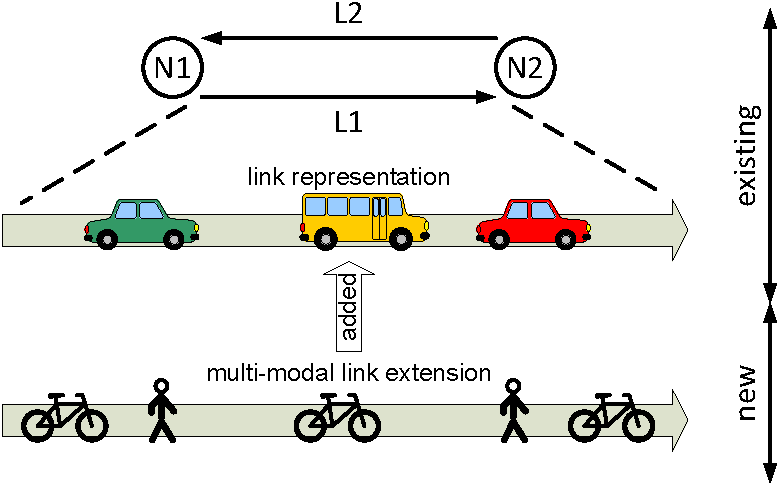
\includegraphics[width=0.5\textwidth, angle=0]{extending/figures/MultiModalSimulation/multi-modal-link-extension} \end{center}

\editdone{This text has undergone the professional edit. Please no grammatical changes anymore! They are most-probably wrong.}

\createStandardInformation{multimodal}{\lstinline|RunMultimodalExample| class}{multimodal}{\citet{00DoblerLaemmelAxhausen2012PedMultiModal}}

% ##################################################################################################################
\section{Introduction}
%There are two basic types of simulation models available in today's agent-based transport simulations. The first type was developed for large-scale scenarios with hundreds of thousands or even several million entities. To keep the computational effort acceptable, this type is based on simplified physical traffic flow representations as identified in a dynamic \gls{trafficassignment} field. In contrast, the second model type offers high detail and a microscopic underlying physics modeling for small scenarios with several hundred or a few thousand agents. While the first type deals only with vehicular traffic, the second generally also deals with pedestrians and cyclists.
%
%A way to reduce the gap between these two simulation types is presented in the following. 

\gls{matsim}'s standard \gls{mobsim}, \gls{qsim}, has recently been enabled to model \gls{multimodal} scenarios as shown in Section~\ref{sec:using-othermodesthancar}. %\kai{chk}

In this chapter,\footnote{Parts of this chapter are based on work published at the 6th International Conference on Pedestrian and Evacuation Dynamics in Zürich \cite{00DoblerLaemmelAxhausen2012PedMultiModal}.}
 an earlier approach to handle \gls{multimodal} scenarios, the \gls{multimodal} link \gls{contribution}, is presented. As shown below, it is a very efficient approach, that considers persons' biking and walking speeds to improve the \gls{teleportation} estimates for these modes, whereas mode interactions are not taken into account. 

%The proposed \gls{multimodal} simulation model adds support for ride trips and non-motorized (i.e., walk and bike) traffic to a framework for large-scale simulations. The next section discusses the requirements of these \gls{multimodal} extensions. Then, modeling approaches for non-motorized and ride trips, as well as their implementation in \gls{matsim}, are described.
%Finally, the implementations are tested by conducting experiments with a sample scenario.

%% ##################################################################################################################
%\section{Requirements}
%Common micro-simulations focusing on vehicular traffic do not provide detailed information about the agents' positions when walking or biking. They either totally ignore non-motorized trips or \gls{teleport} agents from their trips' origins to destinations. When using the latter approach, as \gls{matsim} does so far, travel times are often determined using simple estimation rules, e.g., using an average travel speed and an estimated traveled distance based on the trip's crow-fly distance.
%
%An application's required level of detail strongly influences the modeling approach selection. A simple model including agents' age and gender, but not incorporating agent-agent interactions, might be detailed enough for some studies (e.g., e-bikes or public transport). However, for other studies, a more detailed model, also simulating agent interactions, might be necessary (e.g., evacuation of crowded pedestrian areas).
%
%A model's computational effort increases with its level of detail. Therefore, to keep computation times short, a model should only be as detailed as necessary. One solution is to provide several models with various levels of detail and selecting an appropriate one. On the other hand, a flexible model with an adaptive level of detail can be used. While the latter are more complex, they can provide more detail where needed and can be more aggregated where possible.
%
%One of few implementations of a model with different detail levels of detail is presented by \citet{SewallJEtAl_ACMTG_2011}. They use a hybrid model of both continuum and agent-based methods for vehicular traffic simulations. In regions of interest, the simulation uses an agent-based approach, in other areas a faster continuum model.
%
%For some applications, it is necessary for agents using different transport modes to interact. When modeling such interactions, it is important that infrastructure which would be shared in the real world is also shared in the simulation, to keep the simulation's behavior consistent. An example is shared trip simulation. When sharing infrastructure, an agent performing a ride trip physically enters a vehicle and reduces its free capacity. Therefore, the agent has to wait until the vehicle has arrived and then check whether it has free capacity left. Moreover, the vehicle can wait at the meeting point if the agent to be picked up has not yet arrived.
%
%When not sharing infrastructure, the simulation module for ride trips has to observe all vehicles and track their passengers and capacities. However, a vehicle will not recognize when a passenger has not yet arrived, because it does not communicate with the ride simulation module. As a result, the vehicle will depart and the passenger will not be able to perform its scheduled ride trip. An advantage of this approach is that a ride simulation module could be developed without changing code in the vehicular simulation module.
%
%Compared to vehicular traffic flow simulations, non-vehicular simulations require different input data. An agent's age and gender, for example, strongly influence its walk speed, but this is not taken into account by vehicular traffic flows models. Models including agent-agent or agent-environment interactions also need detailed information about a road network's geometry (e.g., shape, width and height profile of links), as well as buildings and other obstacles in the simulated area.

% ##################################################################################################################
\section{Modeling Approach and Implementation}
% =========================================================================
\subsection{Multi-modal Link Contribution} 
\label{sec:Multi-modalSimulation}
%For the simulation of non-motorized trips a new simulation module has been developed for \gls{matsim}'s \gls{qsim}. 
Figure~\ref{fig:multi-modal-link-extension} shows the implementation's basic concept---a \gls{multimodal} contribution is added to each link object in the \gls{mobsim}. 
% The existing network infrastructure is re-used, which---as discussed before---simplifies the realization of interactions between agents using different transport modes. \ah{But we do not do taht, right?}

%---------------------------------------------------------------------
\createfigure%
{Multi-modal link contribution}%
{Multi-modal link contribution}%
{\label{fig:multi-modal-link-extension}}%
{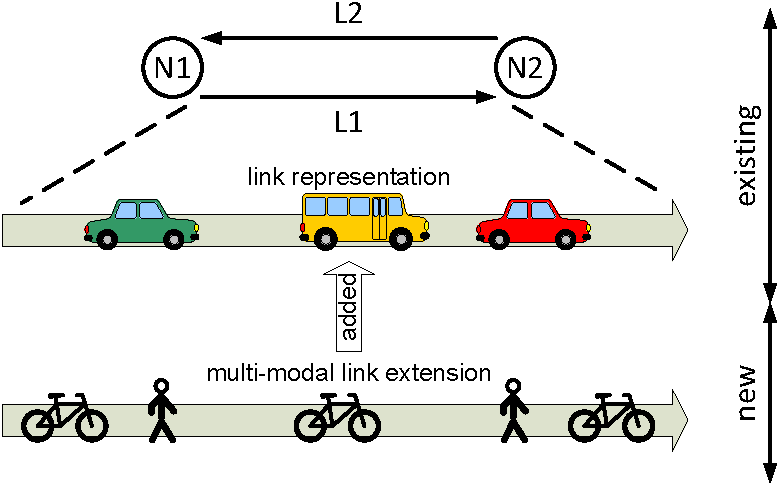
\includegraphics[width=0.75\textwidth, angle=0]{extending/figures/MultiModalSimulation/multi-modal-link-extension}}%
{}
%---------------------------------------------------------------------

While traffic flow dynamics are simulated by \gls{matsim}'s \gls{mobsim} using a queue model, these flows are not taken into account in the \gls{multimodal} contribution. Examining typical pedestrian and cyclist traffic flows shows that congestion is very rare compared to vehicular traffic, justifying application of this simplistic approach over a scenario. For regions with higher traffic flows, this simple model loses accuracy, but still outperforms the \gls{teleportation} approach, which \gls{matsim} uses by default.

Each \gls{multimodal} link contribution uses a priority queue to manage all agents traveling on that link using a non-motorized mode. The queue orders the agents based on their scheduled link leave time (see Figure~\ref{fig:linkRepresentationSimpleModel}). This time is calculated when an agent enters a link and is based on parameters like the agent's age and gender, as well as the links' steepness. In each time step, it is checked whether the queue contains agents who have reached their link leave time and thus must be moved to their route's next link. An agent's position on a link is not determined by the model. However, under the assumption that agents move with constant speed, their position can be interpolated. This approach is computationally very efficient, because computation effort is created only when an agent enters or leaves a link but not when it is traveling along a link. Additionally, agents can travel at different speeds, so can overtake each other.

%---------------------------------------------------------------------
\createfigure%
{Link representation in the simple model}%
{Link representation in the simple model. \\At time 12\,084\,seconds from midnight, agent~512 enters the link and is---based on its calculated link leave time 14\,618\,seconds from midnight---inserted into the queue. At time 12\,312\,seconds from midnight, agent~780 has reached its leave time and is then removed from the queue.}%
{\label{fig:linkRepresentationSimpleModel}}%
{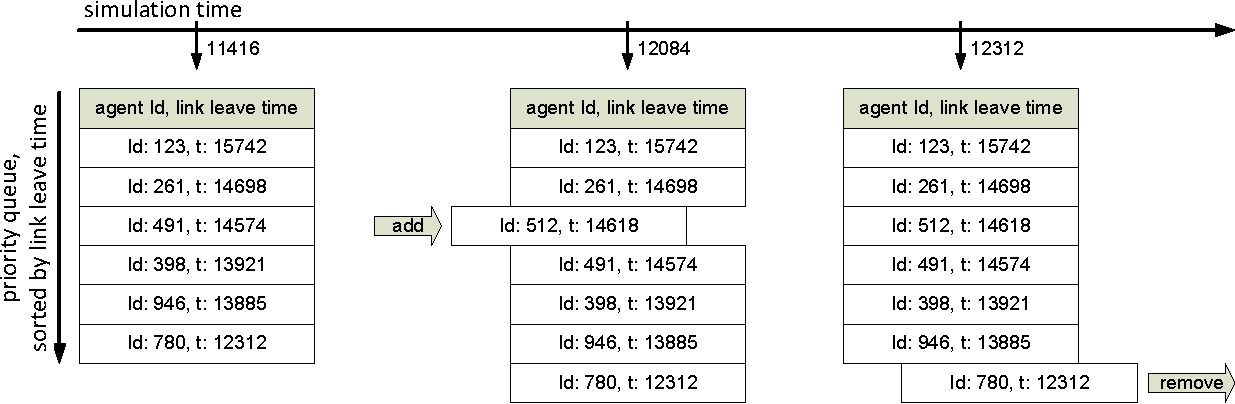
\includegraphics[width=1.0\textwidth, angle=0]{extending/figures/MultiModalSimulation/linkRepresentation}}%
{}
%---------------------------------------------------------------------

% =========================================================================
\subsection{Travel Times} 
\label{sec:TravelTimes}
Walk travel time calculation is based on results of a comprehensive literature review by \citet{Weidmann_TechRep_IVT_1992}. Starting point is a normally distributed reference speed of 1.34\,meters per second with a standard deviation of 0.26\,meters per second, which leads to an individual reference speed for each person. \citet{HBS_2009} and \citet{HCM_2010} report comparable, but less detailed data. If a trip's purpose is known, a person's reference value can be adjusted \citep[commuting 1.49\,meters per second, shopping 1.16\,meters per second, leisure 1.10\,meters per second; see][]{HBS_2009}. Using the reference speed and referencing a person's age, gender and statistical spreading, a personalized speed is calculated (see Figure~\ref{fig:labelPedestriansAge}). Finally, to calculate the person's travel time on a specific link, influence of the link's steepness on the person's speed is taken into account (see Figure~\ref{fig:labelPedestriansSteepness}). The combination of person-specific attributes and link steepness is shown in Figure~\ref{fig:labelPedestriansAgeSteepness3d}.

As a result, a person's speed on plain terrain is calculated as:\begin{align}
	f\textsubscript{person} = f\textsubscript{statistical~spreading} \cdot f\textsubscript{gender} \cdot f\textsubscript{age}\\
	v\textsubscript{person, walk} = v\textsubscript{reference, walk} \cdot f\textsubscript{person}
\end{align}
A link's steepness is incorporated as:
\begin{align}
    v\textsubscript{person~walks~on~link} &= v\textsubscript{person, walk} \cdot f\textsubscript{steepness}
\end{align}

%---------------------------------------------------------------------
\createfigure%
{Age and steepness dependent speed of pedestrians}%
{Age and steepness dependent speed of pedestrians}%
{\label{fig:labelWalkTravelTimes}}%
{%
  \createsubfigure%
  {Age dependent speed}%
  {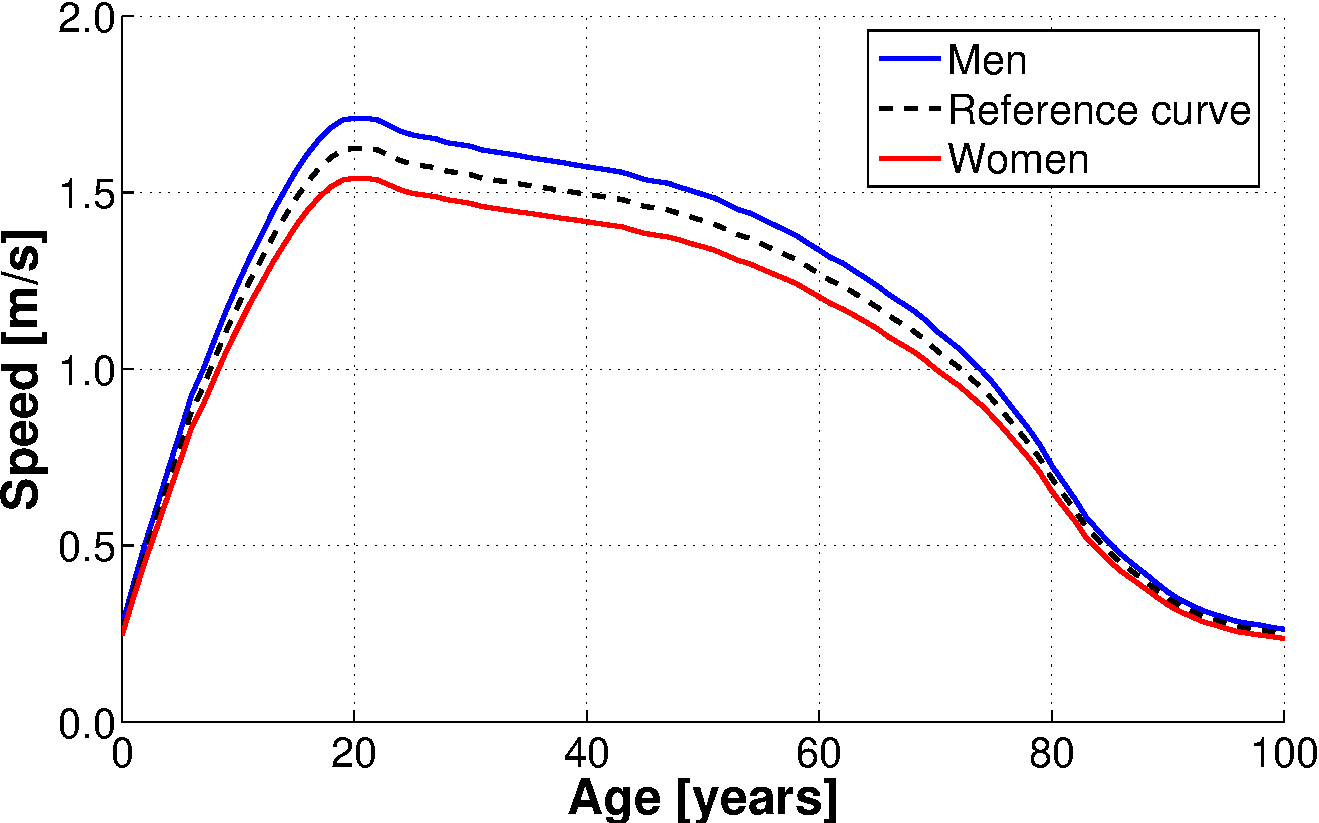
\includegraphics[width=0.65\textwidth, angle=0]{extending/figures/MultiModalSimulation/pedestriansAge}}%
  {\label{fig:labelPedestriansAge}}%
  {\vspace{3mm}}%

  \createsubfigure%
  {Steepness dependent speed}%
  {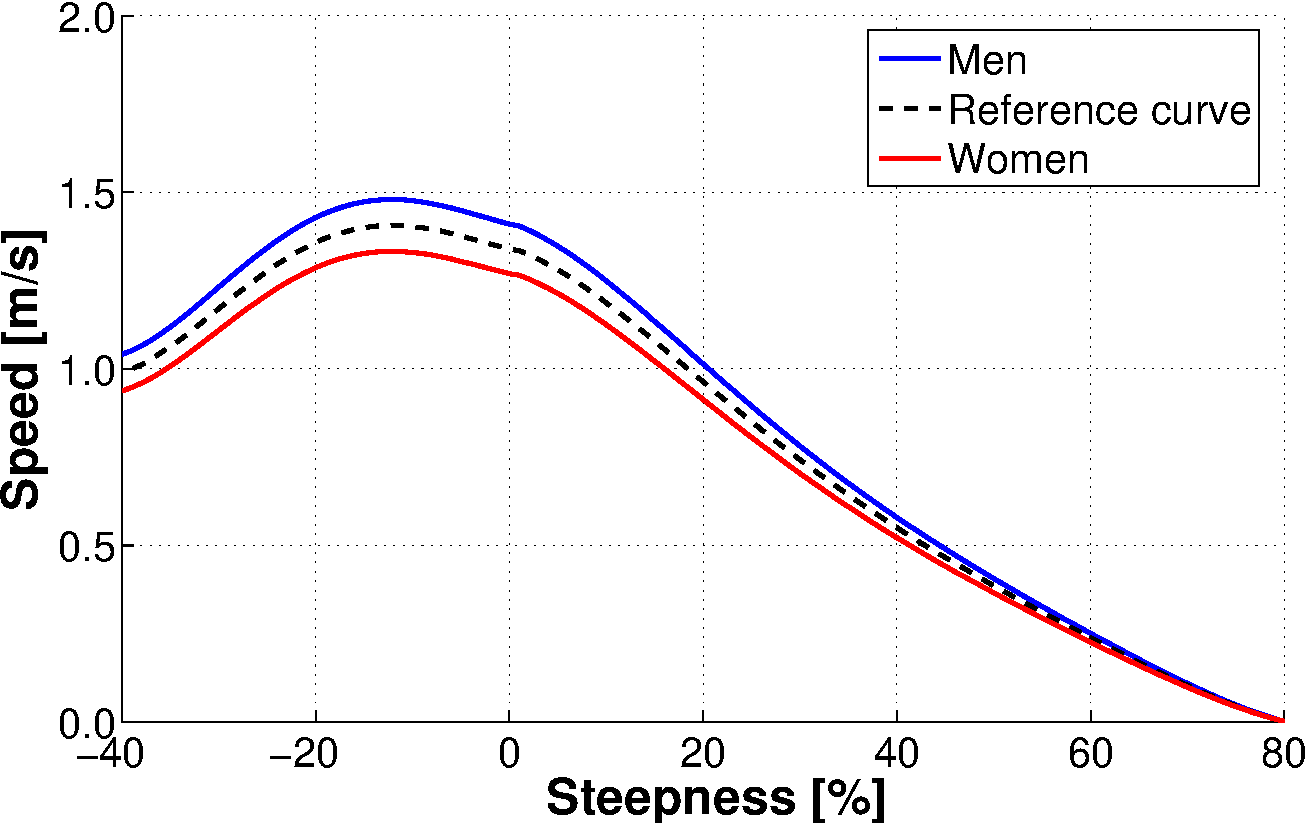
\includegraphics[width=0.65\textwidth, angle=0]{extending/figures/MultiModalSimulation/pedestriansSteepness}}%
  {\label{fig:labelPedestriansSteepness}}%
  {\vspace{3mm}}%

  \createsubfigure%
  {Age and steepness dependent speed}%
  {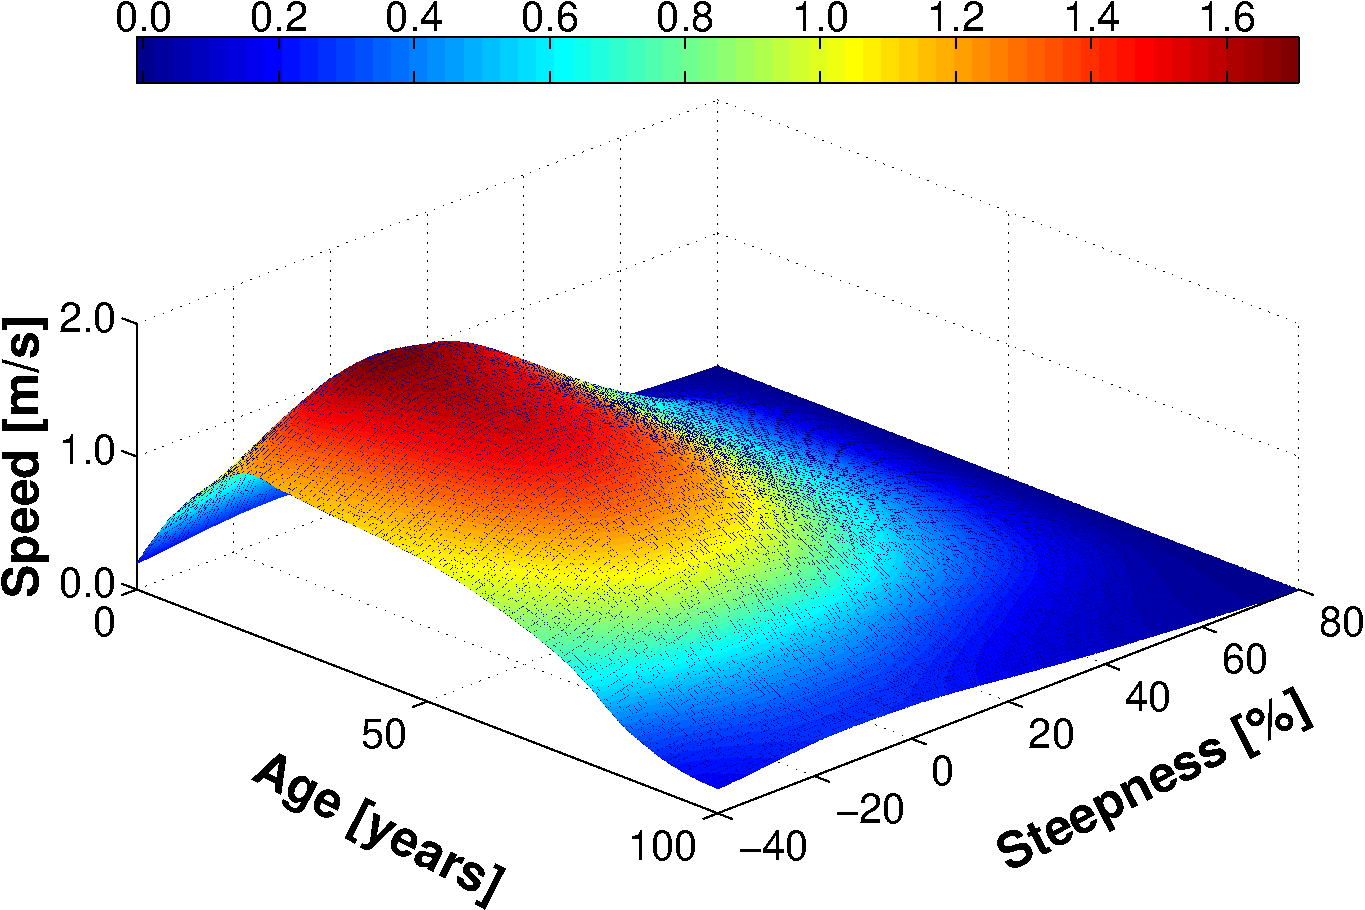
\includegraphics[width=0.65\textwidth, angle=0]{extending/figures/MultiModalSimulation/pedestrians3d}}%
  {\label{fig:labelPedestriansAgeSteepness3d}}%
  {}%
}%
{}
%---------------------------------------------------------------------

The speed of cyclists is determined using results from \citet{ParkinRotheram_TPol_2010}. Starting point is, again, an individual's speed based on a normal distributed ($\mathcal{N}(6.01,1.17)$) reference speed. Once more, a person's speed is calculated by accounting for age and gender (see Figure~\ref{fig:labelCyclistsAge}).

%---------------------------------------------------------------------
\createfigure%
{Age and steepness dependent speed of cyclists}%
{Age and steepness dependent speed of cyclists}%
{\label{fig:labelBikeTravelTimes}}%
{%
  \createsubfigure%
  {Age dependent speed}%
  {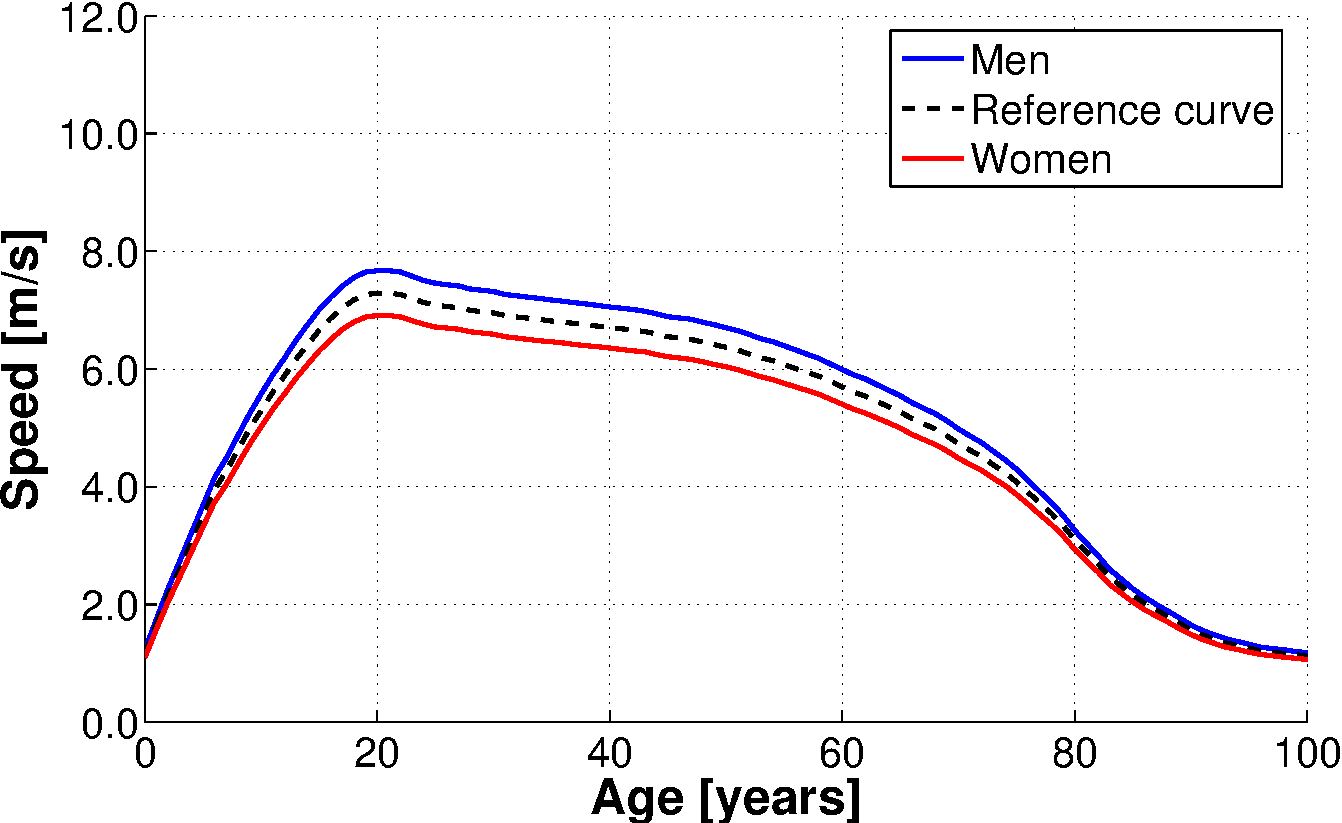
\includegraphics[width=0.65\textwidth, angle=0]{extending/figures/MultiModalSimulation/cyclistsAge}}%
  {\label{fig:labelCyclistsAge}}%
  {\vspace{5mm}}%

  \createsubfigure%
  {Steepness dependent speed}%
  {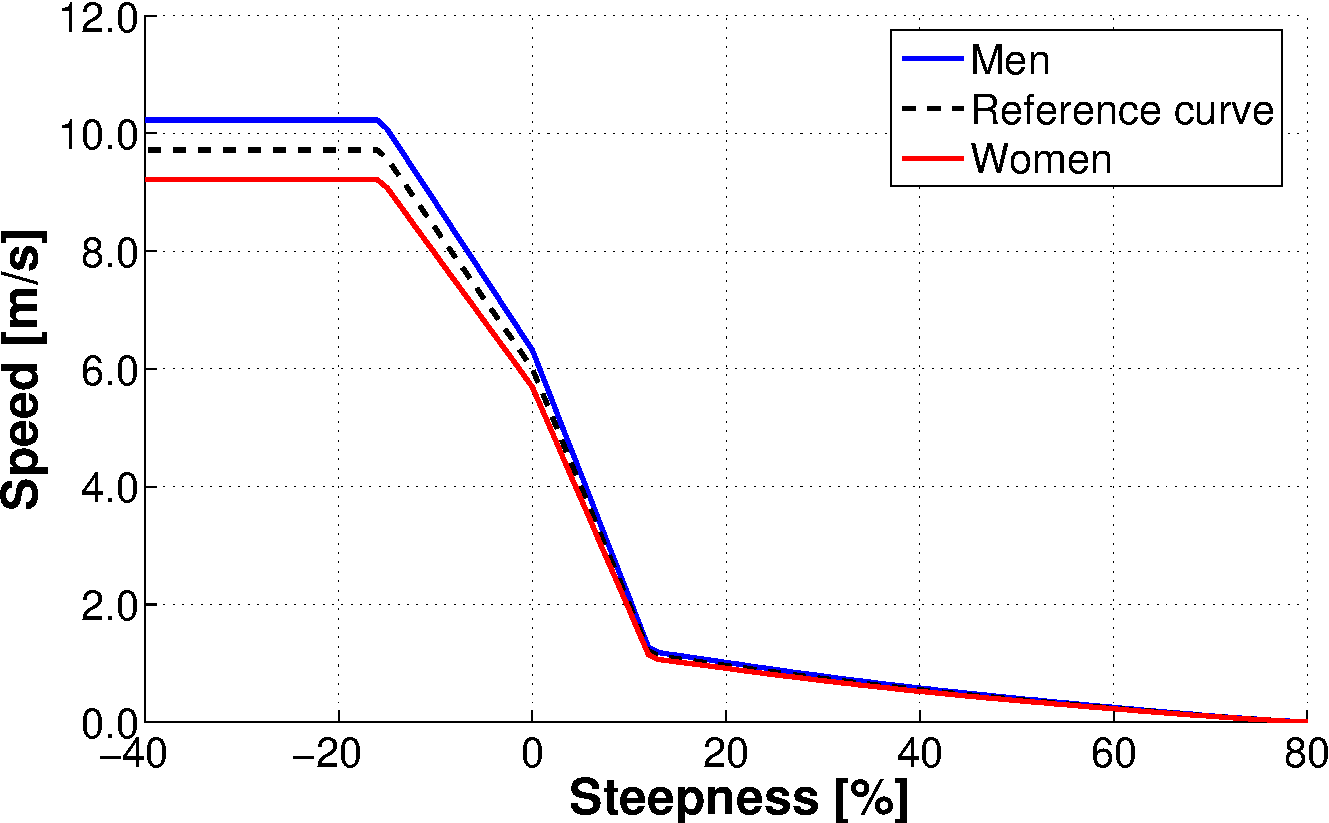
\includegraphics[width=0.65\textwidth, angle=0]{extending/figures/MultiModalSimulation/cyclistsSteepness}}%
  {\label{fig:labelCyclistsSteepness}}%
  {\vspace{4mm}}%

  \createsubfigure%
  {Age and steepness dependent speed}%
  {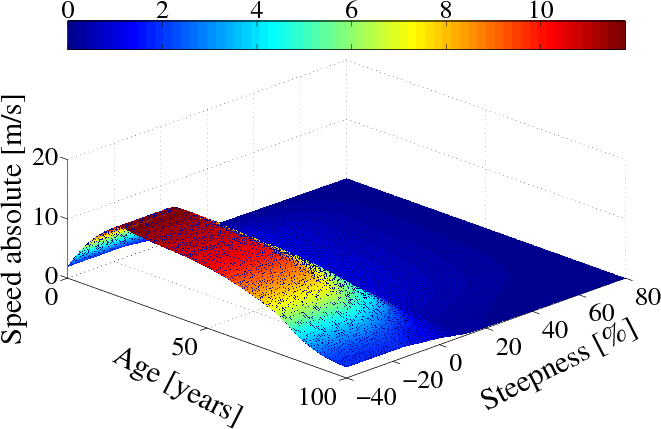
\includegraphics[width=0.65\textwidth, angle=0]{extending/figures/MultiModalSimulation/cyclists3d}}%
  {\label{fig:labelCyclistsAgeSteepness3d}}%
  {}%
}%
{}
%---------------------------------------------------------------------
\afterpage{\clearpage}	% force latex to place the figures somewhere near here and not at the end of the chapter

When calculating the steepness factor, one must define whether a link goes uphill or downhill. When going uphill, the person's speed is reduced by a factor based on the grade and a reference factor of~0.4002\,meters per second, which is scaled by the same factor as the person's reference speed. \ie the speed drop of slow people is lower than the drop of fast people. When bike speed drops below walk speed, which happens at a grade of approximately 12\,\%, it is assumed that the person switches to walking (see Equation~(\ref{equ:bike_uphill})). For downhill links, a reference factor of 0.2379\,m/s is used. Additionally, it is assumed that cyclists limit their speed to 35\,kilometers per hour (9.7222\,meters per second; see Equation~(\ref{equ:bike_downhill})).

% default seems to be ~14.0
{\fontsize{12.8pt}{12}
\begin{align}
    v\textsubscript{person, bike} &= v\textsubscript{reference, bike} \cdot f\textsubscript{person}\\
    v\textsubscript{person, uphill} &= \text{max}
    \begin{cases}
        v\textsubscript{person, bike, flat} - 0.4002 \cdot |\text{grade}| \cdot f\textsubscript{person}\\
        v\textsubscript{person, walk, uphill}
    \end{cases}\label{equ:bike_uphill}\\
    v_{\textsubscript{person, downhill}} &= \text{min}
    \begin{cases}
        v\textsubscript{person, bike, flat} + 0.2379 \cdot |\text{grade}| \cdot f\textsubscript{person}\\
        9.7222
    \end{cases}\label{equ:bike_downhill}
\end{align}
}%

Another parameter affecting pedestrian and cyclist speed is the crowd density of the link where they are physically present. Data to take this effect into account is, again, presented by \citet{Weidmann_TechRep_IVT_1992}. However, to calculate crowd density of a link, its geometry has to be taken into account, as discussed by \citet{Laemmel_PhDThesis_2011}. 

% ##################################################################################################################
\section{Conclusions and Future Work}
The \gls{multimodal} \gls{contribution} allows the tracking an agent's movement in detail, essential for studies related to topics like evacuations, e-bikes, car sharing or public transport. Experiments testing the implementation and demonstrating its capabilities are described by \citet{Dobler_PhDThesis_2013}.

An application's required level of detail strongly influences the modeling approach selection. A simple model including agents' age and gender, but not incorporating agent-agent interactions, might be detailed enough for some studies (\eg e-bikes or public transport). However, for other studies, a more detailed model, also simulating agent interactions, might be necessary. 

A first implementation of a pedestrian simulation module for \gls{matsim}, which also supports agent-agent interactions, was presented by \citet{00LaemmelPlaue2012CollisionAvoidingModels} introducing a force-base model. The agents' high-level planning (\ie route and destination choice) was performed on a graph representing the transport system (\eg a \gls{matsim} network), while the low level behavior (\ie physical interaction between the participants) was simulated with a force-based model. Due to the intense computational effort of the underlying physical model, the scenario size was limited to a few thousand agents. An attempt to bypass this limitation was presented by \citet{00DoblerLaemmel2012MultiModalEvac}. They combined the force-based pedestrian simulation module with the \gls{multimodal} link contribution, creating the opportunity to simulate \gls{largescale} scenarios, by staying highly resolved where needed and being more aggregated where possible.

% ##################################################################################################################
